\chapter{Introducción}

% =============================================================================
% ¿Qué se hizo?
% =============================================================================
En este trabajo se obtuvo un diseño preliminar de la geometría de los  sistemas
de intercambio de gases del  \gls{mrcvc} \cite{toth}, con el objetivo de
maximizar el rendimiento volumétrico en un rango de velocidades.

% =============================================================================
% ¿Cómo se hizo?
% =============================================================================
La optimización se realizó utilizando en conjunto una serie de herramientas de
simulación, las principales fueron: ICESym \cite{icesym}, un simulador de
motores de combustión interna y OpenFOAM \cite{openfoam}, la herramienta libre
de CFD.

Además, se desarrolló un sencillo optimizador capaz de generar y evaluar
diferentes geometrías para buscar la combinación de diámetro, posición y tamaño
de puertos que maximice el rendimiento volumétrico del motor para un rango de
velocidades.


Se realizó una primer aproximación utilizando coeficientes de descarga ($C_{d}$)
estimados en trabajos anteriores \cite{lopez13}, con los cuales se evaluó el
funcionamiento del los parámetros que definen la geometría de los sistemas de
intercambio de gases, en particular diámetros, longitudes y reglaje o posición
angular de los mismos.

Utilizando el algoritmo genético se evaluó una gran cantidad de geometrías
diferentes, dando puntaje a cada una luego de simular el ciclo operativo del
motor y comparar las curvas de rendimiento volumétrico obtenidas con una curva
objetivo, cuanto más parecida la curva de cada motor con dicha curva, mayor
puntaje obtiene una determinada configuración.


El diseño preliminar se volcó en un modelo de CAD de los puertos, con los cuales
se realizó una serie de flujometrías en distintas posiciones del conjunto
rotante, con el fin de obtener un mapa del coeficiente de descarga en
función de dos variables: ``alzada'' equivalente y diferencia de presión.
%
Este mapa de $C_{D}$ se utilizó como retroalimentación del simulador ICESym
para repetir los pasos descritos anteriormente y así obtener un diseño
satisfactorio.

% =============================================================================
% ¿Por qué se hizo?
% =============================================================================
La motivación de este trabajo surge del deseo de continuar con el desarrollo
del MRCVC, en particular mejorar el pre diseño de los sistemas de intercambio de
gases sentando las bases para una futura optimización de los mismos en un motor
con requisitos de diseño establecidos.
%
El MRCVC es un proyecto que surgió en la Universidad Nacional del Comahue,
inventado y patentado por Jorge Toth\cite{toth} en el año 2004, este proyecto
nace en el marco del \emph{Proyecto de Investigación Desarrollo de modelos y
    herramientas para la simulación de problemas complejos en ingeniería
mediante fluido dinámica computacional (04/I-251)}. Actualmente se encuentra en
etapa de desarrollo.

\begin{figure}
    \centering
    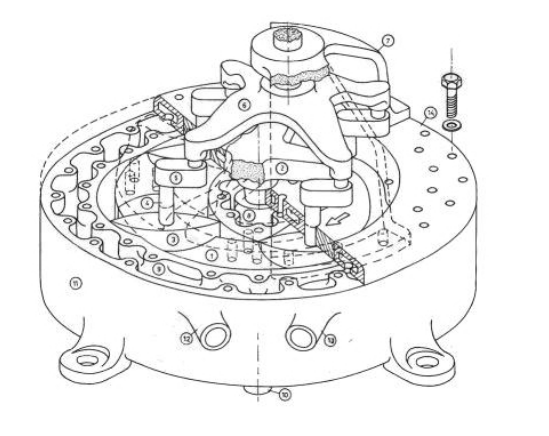
\includegraphics[width=0.5\textwidth]{perspectiva_mrcvc.png}
    \caption{Motor Rotativo de Combustión a Volumen Constante}
    \label{fig:mrcvc}
\end{figure}
